\documentclass[11pt]{article}
\usepackage{classTools}
\usepackage{graphicx}
\drafttrue

\begin{document}

% To include a problems set header, use the psHeader command
\psHeader{4}{Wed Oct. 12, 2022 (11:59pm)}

\textbf{Your name: Nikhil Datar}

\textbf{Collaborators: }

\textbf{No. of late days used on previous psets: 1}

\textbf{No. of late days used after including this pset: 4}

\begin{enumerate}
    \item (Randomized Algorithms in Practice)  
    \begin{enumerate}
        \item Implement Randomized QuickSelect, filling in the template we have given you in the \href{https://github.com/Harvard-CS-120/cs120/tree/main/fall2022/psets}{Github repository}.  
        
        \item 
        In the repository, we have given you datasets $x_n$ of key-value pairs of varying sizes to experiment with.  For each dataset $x_n$ and any given number $k$, you will compare two ways of answering the $k$ selection queries
        Select$(x_n,[n/k])$, Select$(x_n,[2n/k]), \ldots$, Select$(x_n,[(k-1)n/k])$ on $x_n$, where $[\cdot]$ denotes rounding to the nearest integer:
        \begin{enumerate}
            \item Running Randomized QuickSelect $k$ times
            \item Running MergeSort (provided in the repository) once and using the sorted array to answer the $k$ queries
        \end{enumerate}
        Specifically, you will compare the {\em distribution} of runtimes of the two approaches for a given pair $(n,k)$ by running each approach many times and creating density plots of the runtimes.  The runtimes will vary because Randomized QuickSelect  is randomized, and because of variance in the execution environment (e.g. what other processes are running on your computer during each execution).
        
        We have provided you with the code for plotting. Before plotting, you will need to implement MergeSortSelect, which extends MergeSort to answer $k$ queries. Your goal is to use these experiments and the resulting density plots to propose a value for $k$, denoted $k^*_n$, at which you should switch over from Randomized QuickSelect to MergeSort for each given value of $n$. Do this by experimenting with the parameters for $k$ (code is included to generate the appropriate queries once the $k$s are provided) and generate a plot for each experiment.  Explain the rationale behind your choices, and submit a few density plots for each value of $n$ to support your reasoning.  (There is not one right answer, and it may depend on your particular implementation of QuickSelect.) \\
        
        SOLUTION: Given that $k$ is the number of times QuickSelect runs and queries in MergeSort, and the fact that we want to find the values of $k$ at which MergeSort becomes faster than QuickSelect, we must choose values of $k$ such that the distributions of the runtimes roughly overlap. This would be a clear indicator of where MergeSort overtakes QuickSelect. \\
        
        \begin{tabular}{ | m{5em} | m{1cm}| m{1cm} | } 
  \hline
  N & K  & EQ\\ 
  \hline
  2048 & 20 & $\log 2048 + 9 = 20$\\ 
  \hline
  4096 & 22 & $\log 4096 + 10 = 22$ \\ 
  \hline
  8192 & 24 &  $\log 8192 + 11 = 24$ \\
  \hline
  16384 & 26 &  $\log 16384 + 12 = 26$ \\
  \hline
  32768 & 28 &  $\log 32768 + 13 = 28$ \\
  \hline
\end{tabular} \\

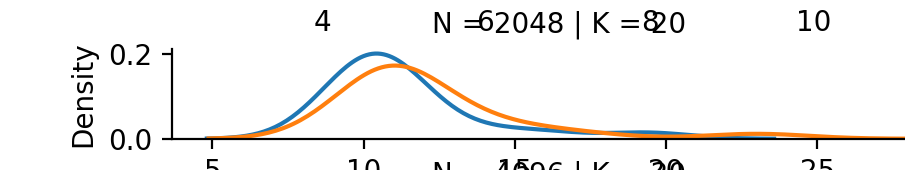
\includegraphics[width = \textwidth]{k=20}\\
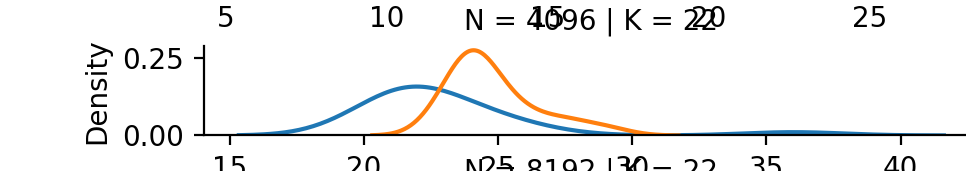
\includegraphics[width =\textwidth]{k=22}\\
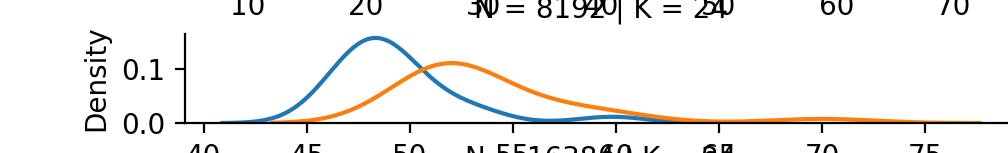
\includegraphics[width = \textwidth]{k=24}\\
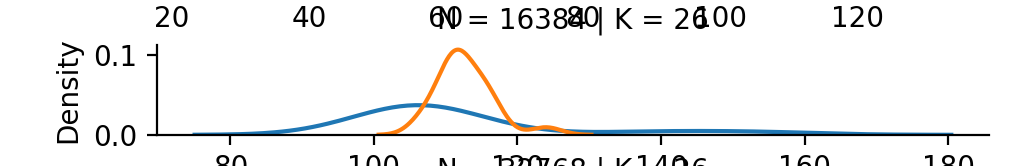
\includegraphics[width = \textwidth]{k=26}\\
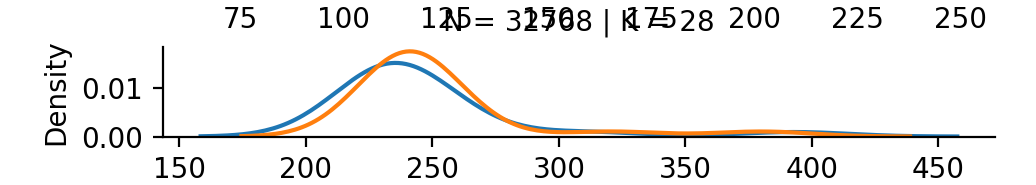
\includegraphics[width = \textwidth]{k=28}\\

        \item Extrapolate to come up with a simple functional form for $k^*_n$, e.g. something like $k^*(n)=3\sqrt{n}+6$ or $k^*(n)=10\log n$. (Again there is not one right answer.) \\
        
        From the values of $k$ and graphs above, we showed that the constant that was needed to add to $\log N$ to equal $k$ was roughly $11$. Thus, since we can extrapolate and calculate $k^*_n$ the same way as we did in the table, we have 
        $$
        k^*_n = \log N + 11.
        $$

        \item (*optional)  One way to improve Randomized QuickSelect is to choose a pivot more carefully than by picking a uniformly random element from the array. A possible approach is to use the \textit{\textbf{median-of-3}} method: choose the pivot as the median of a set of 3 elements randomly selected from the array. Add Median-of-3 QuickSelect to the experimental comparisons you performed above and interpret the results.
    \end{enumerate}


    \item (Dictionaries and Hash Tables) 
    Recall the DuplicateSearch problem from Lecture 3. Show that DuplicateSearch can be solved by a Las Vegas algorithm with expected runtime $O(n)$ using a dictionary data structure.  (You can quote the runtimes of the implementation of a dictionary data structure from Lecture 9 without proof.) \\
    
    SOLUTION: We wish to find a duplicate element of an input array if it exists. We will show that a Las Vegas algorithm can be used in conjunction with a dictionary, or Hash Table data structure, in order to solve this problem in $O(n)$ time. \\
    
    Preprocess($U$, $m$): First, we must preprocess. We initialize an array $A$ of size $m$, as well as a random hash function $h: U \to m$ that maps elements from a universe $U$ to a universe $m$. Now, because we don't want elements of different values being mapped to the same location, which would cause collisions not representative of duplicates, we must ensure that $m$, the size of $A$, is at least $n$, the number of elements in the input array. Thus, we set $m=n$. \\
    
    Traversal: We now traverse through the elements of the input array. At each element, we call $Search(K)$ where $h(K)$ is a hashed current element corresponding to the element $K$ within the input list. If this doesn't return a value within the table (duplicate), then we must insert the value into the hash table. This requires calling $Insert(K)$ where we insert the element $K$ into a linked list starting at location $A[h(K)]$. Otherwise, if $Search$ was successful and we indeed found the element $K$ within the hash table at $A[h(K)]$, then we simply return $K$ as the duplicate element. \\
    
    Final: At the end of the loop, if no value was returned, then there are no duplicate elements in the input array, and we return nothing. \\
    
    Algorithmic correctness: We know that the $Preprocess$,  $search$, and $Insert$ functions used in this Las Vegas algorithm are already valid function calls of a hash table data structure. First, we know that since the traversal is occurring through the entire input array, we will cover (search/hash, insert/check if exists) every element, and thus will cross a duplicate element if it exists. Because we defined $m =n$ so that there are enough unique positions in $A$ for all the input elements, we know that when an element $K$ is stored at $A[h(K)]$, the only way in which the linked list beginning at index $h(K)$ will have more than one element is if $K$ is a duplicate. If we found this to not be the case, then we know that all elements of the input array were hashed to different indices and thus each linked list in $A$ would only contain one element. This is known as the loop invariant, in which the algorithm makes sure that each element is unique to be hashed to a unique location, and if not, then we would return a duplicate element as desired. \\
    
    Runtime: The preprocessing step to initialize the hash table takes $O(n+m)$ time. Because we defined $m=n$ to ensure unique hashes of non-duplicate elements, this runtime can be simplified to $O(n+n) = O(n)$. Then, for the traversal step, we call both $Search$ and potentially $Insert$. We know that $Search$ is $O(1)$ runtime from lecture, and insert is $O(1 + \frac{n}{m})$. Again, because we defined $m=n$, the runtime of insert simplifies down to $O(1 + \frac{n}{n}) = O(1)$. Thus, $Search$ and $Insert$ take constant time each, and since we call them for at worst every element of the input array, the total runtime of these function calls combined is $O(n)$. Thus, since the worst runtime of any step was $O(n)$, it follows that the runtime of the Las Vegas algorithm we defined herein is simply $O(n)$ overall. 
    
    

    \item  (Rotating Walks)  
    Suppose we are given $k$ digraphs on the same vertex set, $G_0=(V,E_0), G_1=(V,E_1), \ldots, G_{k-1}=(V,E_{k-1})$.  For vertices $s,t\in V$, a {\em rotating walk} with respect to $G_0,\ldots,G_{k-1}$ from $s$ to $t$ is a sequence of vertices $v_0,v_1,\ldots,v_{\ell}$ such that $v_0=s$, $v_\ell=t$, and $(v_i,v_{i+1})\in E_{i \bmod k}$ for $i=0,\ldots,\ell-1$.  That is, we are looking for walks that rotate between the digraphs $G_0,G_1,\ldots,G_{k-1}$ in the edges used.
    \begin{enumerate}
        \item Show that the problem of finding a Shortest Rotating Walk from $s$ to $t$ with respect to $G_0,\ldots,G_{k-1}$ 
        can be reduced to Single-Source Shortest Walks via a reduction that makes one oracle call on 
        a digraph $G'$ with $kn$ vertices and $m_0+m_1+\cdots+m_{k-1}$ edges, where $n=|V|$ and $m_i=|E_i|$.
        We encourage you to index the vertices of $G'$ by pairs $(v,j)$ where $v\in V$ and $j\in [k]$. 
        Analyze the running time of your reduction and deduce that the Shortest Rotating Walk can be found in time $O(kn+m_0+\cdots+m_{k-1})$.
        \label{part:ReduceToOrdinary}  To test your reduction and algorithm, try running through the example in Part~\ref{part:BFS}. \\
        
        Preprocessing: We first need to construct a $G' = (V', E')$ with $kn$ vertices. We then have that $|V'| = kn$, $n = |V|$ and $|E'| = m_0 + m_1 + \dots + m_{k-1}$. We then want to flatten the disconnected graphs. We do this by creating our edges such that each step follows the same path as the original graph, yet is directed to the vertex in the next steps graph. By doing this, all edges can be represented in $G'$, and thus as defined, the number of edges in this graph is simply the total number of edges in the other graphs, which is $m_0 + m_1 + \dots + m_{k-1}$. \\
        
        Oracle: We then make a call to the Single-Source Shortest Walk oracle on $G'$, for some $s'$, which returns the length of the shortest walk to each $s'$ within our graph. \\
        
        Postprocessing: Given that Single-Source Shortest walk returns the distance and shortest path from $s$ to all other vertices that can be reached within our graph $G'$, we simply need to traverse through all of these paths and find the ones mapping $s \to t$. We want to find the shortest one, so if there are more than one paths, then we simply use the distance to return the shortest rotating walk path from $s \to t$. \\
        
        Runtime: \\
        
        Preprocessing: The time for preprocessing is simply the time to create the graph $G'$. Since there are $kn$ vertices and $m_0 + m_1 + \dots m_{k-1}$ edges, it follows that the runtime of this step is O($kn + m_0 + m_1 + \dots m_{k-1})$. \\
        
        From lecture we had that the runtime of the oracle Single-Source Shortest Walk would be $O(n+m)$. Converting this to the current problem, the $n$ and $m$ would translate to the vertices and edges, and thus the runtime is simply O($kn + m_0 + m_1 + \dots m_{k-1})$. \\
        
        Post-process: To identify the shortest path we go through every shortest path from $s$ to all vertices $n$ to get $t$ and then return the shortest $s \to t$. Since we travel through the vertices the runtime is $O(kn)$. \\
        
        Thus, the overall runtime is the maximum of all the individual runtimes, so overrall it is simply $O(kn + m_0 + m_1 + \dots m_{k-1})$ \\
        
        Correctness: First, we know that the graph $G'$ contains all possible paths from the starting vertex to the ending vertices. This is due to the way we initialize $G'$ within the processing step, which deals with the rotations. This is because all rotations can be found within $G'$. Furthermore, we can assume that the oracle Single-Source Shortest Walk returns the correct distance and predecessor array of the shortest walk to the ending vertices. Lastly, the postprocessing step filters for the minimum distance which is simply comparison, so indeed it will return the shortest path from $s \to t$. Thus our algoirthm is correct. 
        
        
        
        \item \label{part:BFS} Run your algorithm from Part~\ref{part:ReduceToOrdinary} on the following pair of graphs $G_0$ and $G_1$ to find the Shortest Rotating Walk from $s=a$ to $t=c$; this will involve solving Single-Source Shortest Walks on a digraph $G'$ with $2\cdot 8=16$ vertices. Fill out the table provided below with the BFS frontier in $G'$ at each iteration, labelling the vertices of $G'$ as $(a, 0),(b, 0),\ldots,(g,0),(a,1),(b,1),\ldots,(g,1)$, and for each vertex $v$ in the table, drawing an arrow in the graph from $v$'s BFS predecessor to $v$. 
%        \salil{is this the same example as from last year?  May be good to change it.} \salil{where's the table?}

            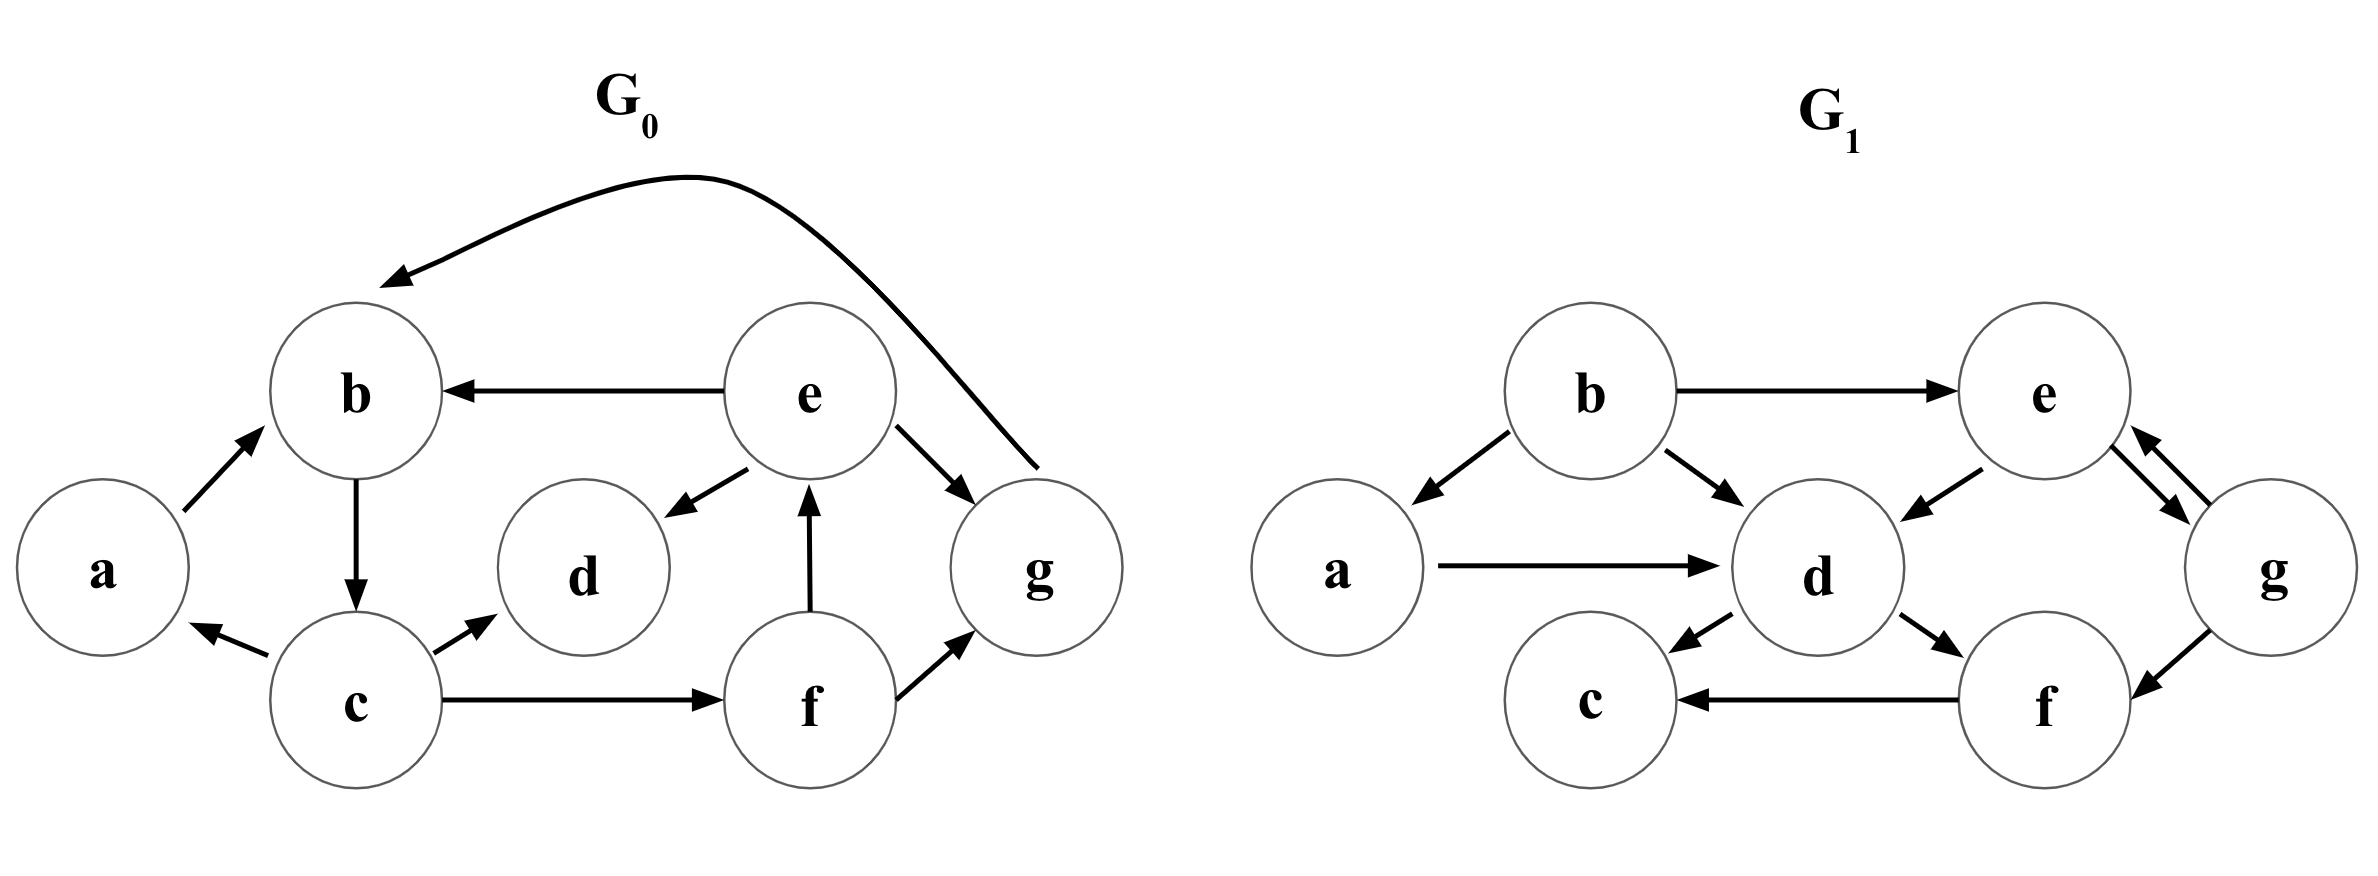
\includegraphics[width=14cm]{ps4_graphs_new.png}

        \begin{table}[ht]
        \centering
        \begin{tabular}{c|c|c}
            $d$ & Frontier $F_d$& Predecessor Relationships \\
            \hline
             0 & (a,0)& N/A\\
             1 & (b, 1)& (a, 0) \to (b, 1)\\
             2 & (d, 0), (e, 0)&  (b, 1) \to (d, c); (b, 1) \to (e, 0)\\
             3 & (d, 1), (g, 1)& (e, 0) \to (g, 1); (e, 0) \to (d, 1)\\
             4 & (c, 0), (f, 0)& (d, 1) \to (f, 0); (d, 1) \to (c, 0)\\
        \end{tabular} \\
        
From this table we can see that the shortest rotating walk from $a$ to $c$ is of length 4. 
    \end{table}
    \item 
        A group of three friends decides to play a new cooperative game (similar to the real-life board game Magic Maze).  They rotate turns moving a shared single piece on an $n\times n$ grid.  The piece starts in the lower-left corner, and their goal is to get the piece to the upper-right corner in as few turns as possible.  Many of the spaces on the grid have visible bombs, so they cannot move their piece to those spaces.  Each player is restricted in how they can move the piece.  Player 0 can move it like a chess-rook (any number of spaces vertically or horizontally, provided it does not cross any bomb spaces). Player 2 can move it like a chess bishop (any number of spaces diagonally in any direction, provided it does not cross any bomb spaces).  Player 3 can move it like a chess knight (move to any non-bomb space that is two steps away in a horizontal direction and one step away in a vertical direction or vice-versa).   Using Part~\ref{part:BFS}, show that given the $n\times n$ game board (i.e., the locations of all the bomb spaces), they can find the quickest solution in time $O(n^3)$.  
        (Hint: give a reduction, mapping the given grid to an appropriate instance $(G_0,G_1,\ldots,G_{k-1},s,t)$ of Shortest $k$-Rotating Paths.) \\
        
        This problem can be simulated as a rotating walk problem between 3 distinct graphs, where each player is represented by one of the graphs. \\
        Preprocessing: Trasform the $n\times n$ grid to a graph. Note that every space in the grid is a vertex in the graph, and we treat all the possible moves from one space to another as the edges within our new graph. Thus, we have succesfully created a graph with each players movements. The problem of the quickst solution on the chessboard can then be reduced to finding the shortest $k$ rotating path where the 3 digraphs are on the same vertex set, represented as $G_0 = (V, E_0), G_1 = (V, E_1)$ and $ G_2 = (V, E_2)$ where $E$ represents the respective edges of the graphs. $s$ is the starting position at the lower left corner of the board and our destination $t$ is at the upper right corner. Since we have correctly defined this we then can use the algorithm given in $3a$ to solve this and find the shortest path. Note that the bombs cover some of these vertices. 
        
        \\ Player0: This player is the rook and there are $2n-2$ squares theye can move to on the board. Thus there are $2n-2$ edges in the worse case and $n^2$ vertices, so the total number of is $n^2(2n-2)$.
        \\Player 1: This player is the bishop and also has $2n-2$ edges and $n^2$ vertices so the number of edges is also $n^2(2n-2)$\\
        
        Player 2: This is the knight, which can make $8$ possibe moves so the total number of edges is simply $n^2 \times 4$. Thus the total runtime is the runtime of the worst possible digraph, so the total runtime is $O(n^2 \times (2n-2)$ or simply $O(n^3)$
    \end{enumerate}
\end{enumerate}
\end{document}
